This chapter describes the design of our application, ... \todo{Other things than the application?}

The reader is expected to be familiar with standard Android components. Some components are briefly explained here:
\begin{description}
\item[Activity] An activity is a single focused thing that the user can do. You can also say that it is a window which is either full-screen or floating. \citep{activity}
\item[Fragment] A fragment inherits from activity and thus has its own lifecycle. Fragments are nested in activities, and can be used to build a multi-pane user interface. \citep{fragment}
\end{description}

\section{Application Design}\label{sec:appdesign}

Before designing a prototype of our application we looked at a few other applications to get inspiration for our design.

\begin{figure}[H]
\begin{minipage}[b]{0.5\columnwidth}
\centering
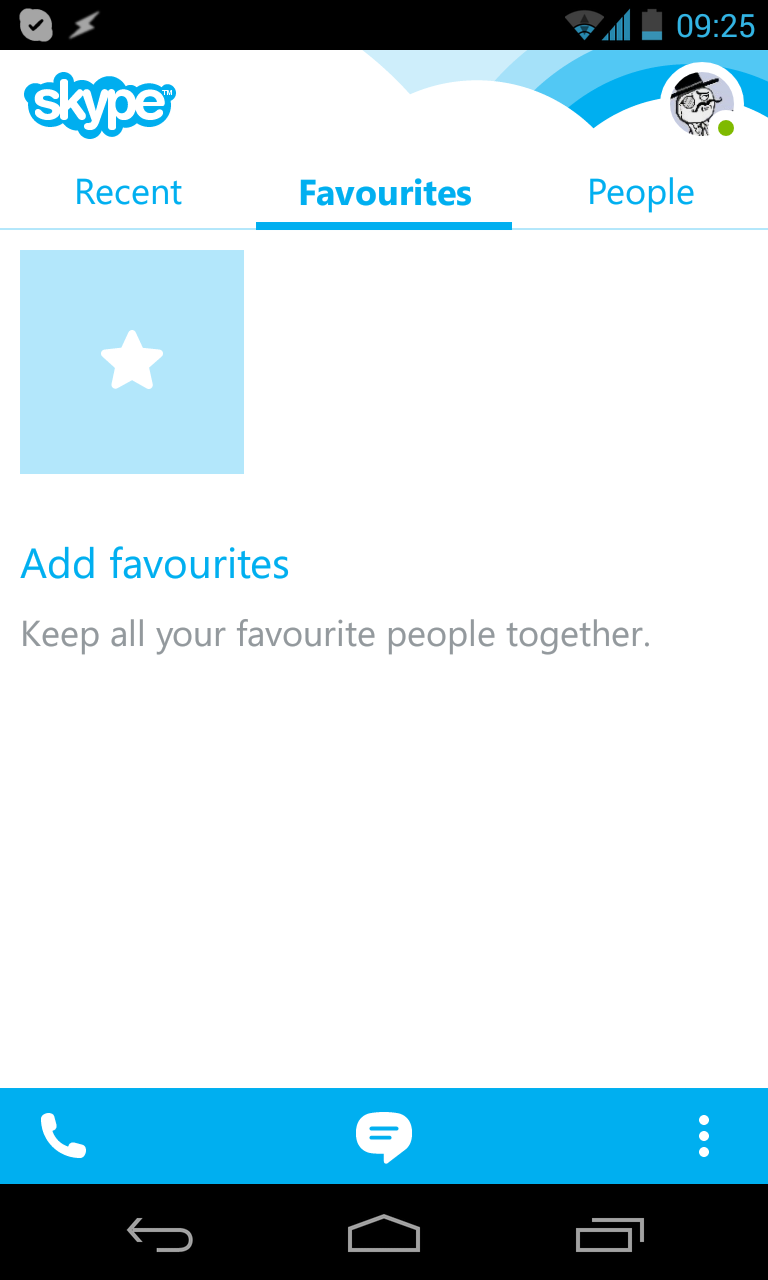
\includegraphics[width=0.7\columnwidth]{img/screenshots/twitter.png}
\caption{Skype\label{fig:skype}}
\end{minipage}
\hspace{0.5cm}
\begin{minipage}[b]{0.5\columnwidth}
\centering
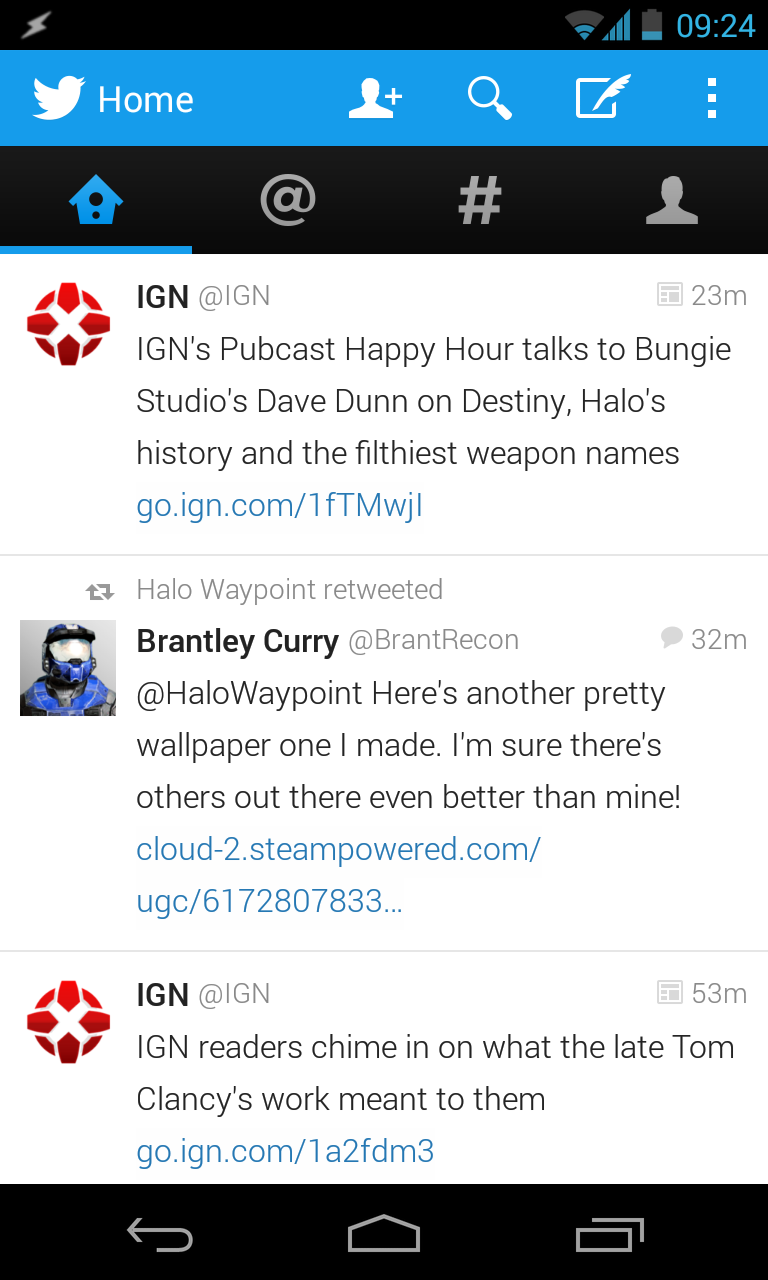
\includegraphics[width=0.7\columnwidth]{img/screenshots/skype.png}
\caption{Twitter\label{fig:twitter}}
\end{minipage}
\end{figure}

We decided that using tabs, like Skype in  \autoref{fig:skype}, was a good way for the user to easily see multiple pages of information by just swiping to the side.

We recognised that we were going to create a few different lists for the application e.g. a list of feeds and a schedule, for this we looked at Twitter \autoref{fig:twitter} and tried to capture their simplicity of tweets in our list items.

\subsection*{Story}
Julie opens our application Exhib. She is presented with a list of exhibitions that she browse. She browses the exhibitions and reads about them, she finds a software exhibition and decides that she want to go there. She clicks the "Floor Plan" tab which shows the exhibitions location. With her smartphone she can use her built-in \ac{gps} application to drive to the exhibition. When she arrives at the exhibition she quickly notices a sign that tells her to scan an \acs{nfc} tag. She scans the \acs{nfc} tag and the system registers a new user. An activity appears asking her what categories and related booths she would like to subscribe to. She picks Microsoft and clicks continue. Now she has access to everything about the exhibition: Exhibition information, map of the exhibition, news feed based on her subscriptions, and a schedule. Julie gets a quick overview of major events in the schedule and the news feed, and then decides to go directly to a Microsoft booth. On the floor plan she finds a Microsoft booth, clicks it, and chose to get directions to the booth. The application remembers Julie's last known location, i.e. the last \acs{nfc} tag she scanned, and generates a route from there to the booth.

\section{Prototype Design}

Here we show our first revision of a prototype for our application. We created this together to reflect, visualise, and agree on the design.

\begin{figure}[H]
\begin{minipage}[b]{0.5\columnwidth}
\centering

\includegraphics[width=0.7\columnwidth]{img/prototype/1.png}
\caption{Start screen\label{fig:start}}
\end{minipage}
\hspace{0.5cm}
\begin{minipage}[b]{0.5\columnwidth}
\centering
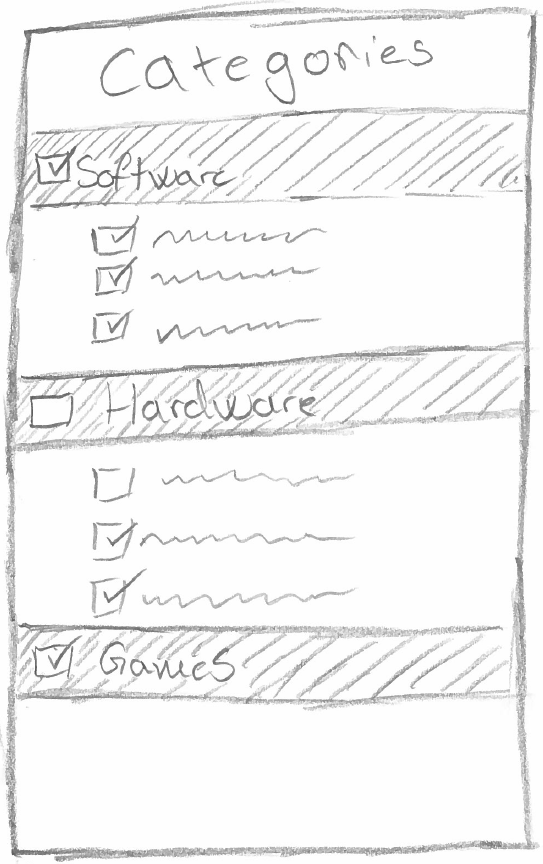
\includegraphics[width=0.7\columnwidth]{img/prototype/2.png}
\caption{Categories\label{fig:categories}}
\end{minipage}
\end{figure}

\autoref{fig:start} shows the application start screen. The user is told to scan an \ac{nfc} tag. When a tag is scanned the application checks if the user has visited the exhibition before. If the user has visited before then the exhibition information is opened, if not, then the user is asked to choose categories.

From the start screen you can also open a small menu in the bottom left corner where the user can browse for exhibitions and also pick recently visited exhibitions.

\autoref{fig:categories} is where you pick categories by clicking the check boxes. Although not present in the picture, the user should click submit in the bottom of the activity.

\begin{figure}[H]
\begin{minipage}[b]{0.5\columnwidth}
\centering
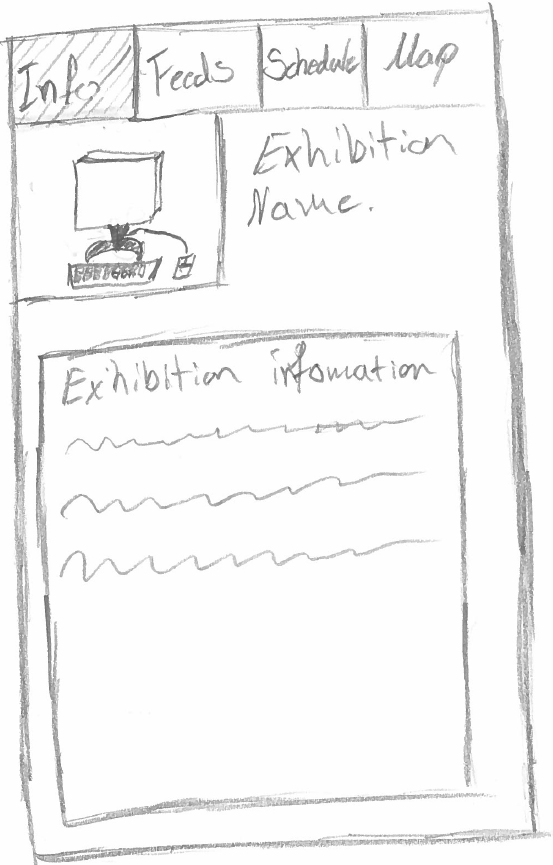
\includegraphics[width=0.7\columnwidth]{img/prototype/3.png}
\caption{Exhibition information\label{fig:exhibition}}
\end{minipage}
\hspace{0.5cm}
\begin{minipage}[b]{0.5\columnwidth}
\centering
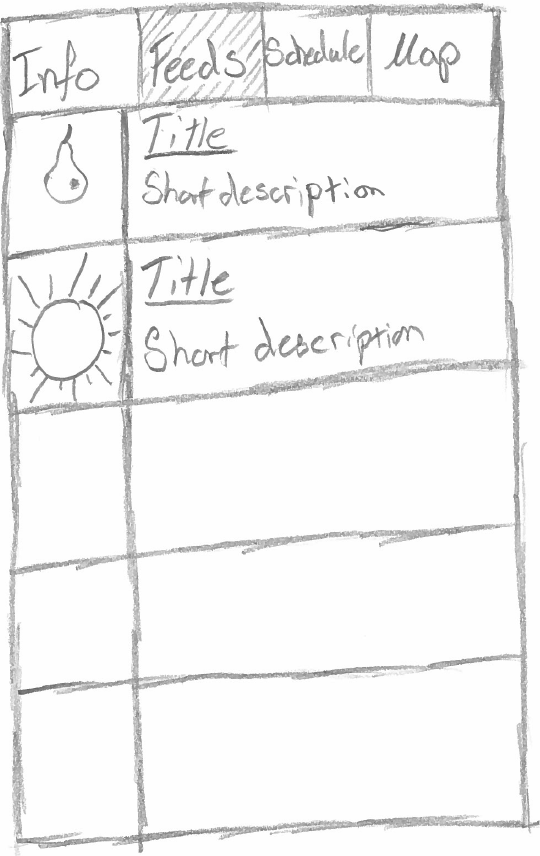
\includegraphics[width=0.7\columnwidth]{img/prototype/4.png}
\caption{Feed list\label{fig:feedlist}}
\end{minipage}
\end{figure}

When you are successfully registered at the exhibition, then you get to the core of the application. Here you can swipe between the different tabs, and also access a specific tab by clicking on it in the top menu. \autoref{fig:exhibition} shows the first tab, notice the tab bar in the top of the application showing which tab you are viewing. This is a simple welcome screen showing the exhibition icon, exhibition name, and an exhibition description.

\autoref{fig:feedlist} shows the feed list associated with the exhibition. The user receives feeds based on the chosen subscriptions that was submitted with the activity in \autoref{fig:categories}. An exhibition can have many feeds, and loading hundreds of feeds at the same time might slow down the application. The feed list should only load a few feeds at a time.

\begin{figure}[H]
\begin{minipage}[b]{0.5\columnwidth}
\centering
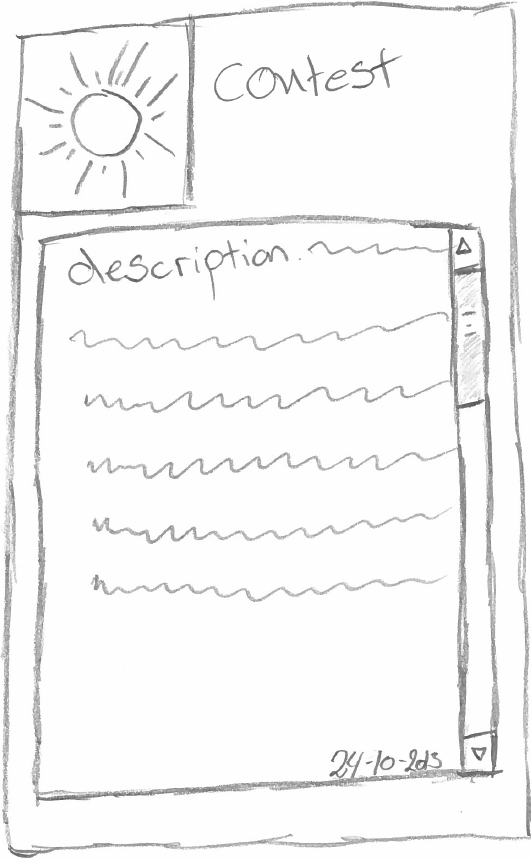
\includegraphics[width=0.7\columnwidth]{img/prototype/5.png}
\caption{Feed item\label{fig:feeditem}}
\end{minipage}
\hspace{0.5cm}
\begin{minipage}[b]{0.5\columnwidth}
\centering
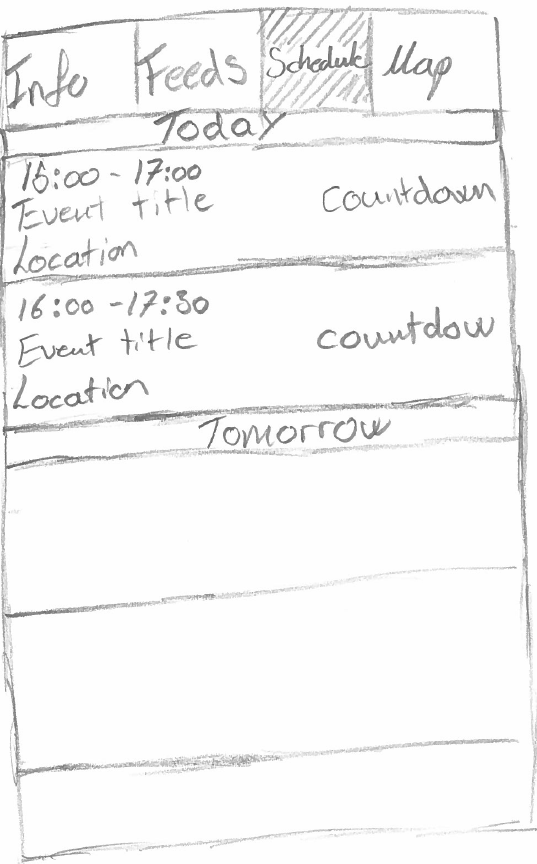
\includegraphics[width=0.7\columnwidth]{img/prototype/6.png}
\caption{Schedule\label{fig:schedule}}
\end{minipage}
\end{figure}

\autoref{fig:feeditem} is the activity shown when you click a feed item from the feed list. A feed item consists of a headline, a feed description, and it shows the icon attached to the booth which is associated with the feed item.

\autoref{fig:schedule} shows the schedule of the exhibition. The schedule items are grouped by days. Each schedule item shows the time interval of the event, a title, a location, and it shows a continuously updated countdown to the event.

\begin{figure}[H]
\begin{minipage}[b]{0.5\columnwidth}
\centering
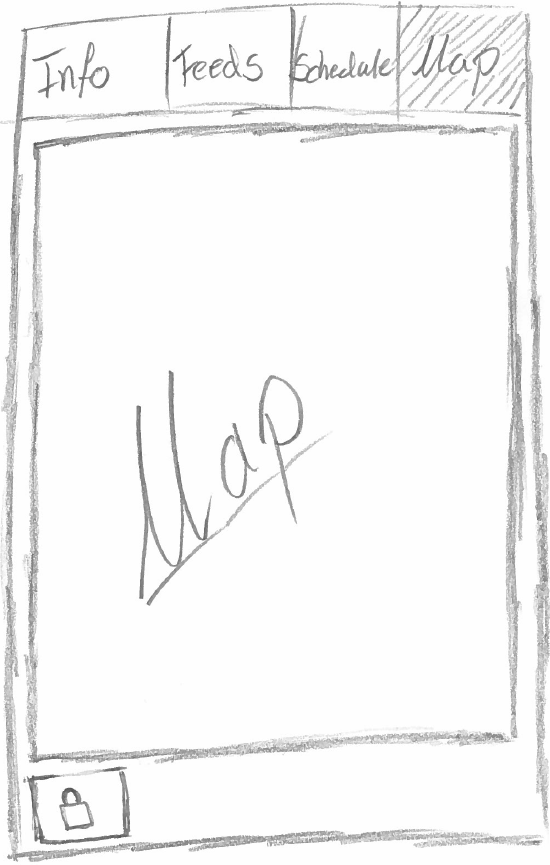
\includegraphics[width=0.7\columnwidth]{img/prototype/7.png}
\caption{Map\label{fig:floorplan}}
\end{minipage}
\hspace{0.5cm}
\begin{minipage}[b]{0.5\columnwidth}
\centering
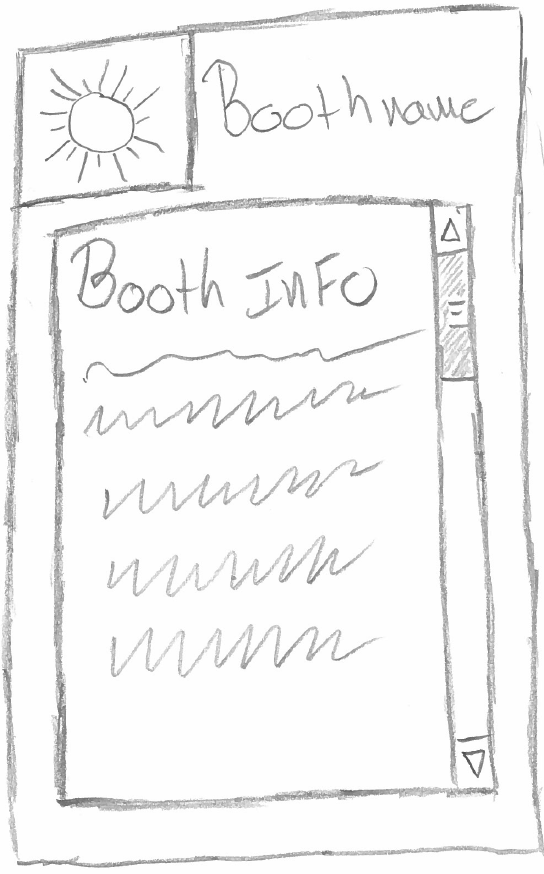
\includegraphics[width=0.7\columnwidth]{img/prototype/8.png}
\caption{Booth information\label{fig:booth}}
\end{minipage}
\end{figure}

\autoref{fig:floorplan} shows the tab displaying the floor plan of the exhibition. Below the map there is a lock button, which locks the user to navigating the floor plan e.g. swiping left and right on the map. If it is not locked then swiping right will change to the schedule tab. Inside the floor plan there should be pinned booths which can be clicked on. When clicking the booths the activity shown in \autoref{fig:booth} is opened. The booth activity shows its attached icon, a name, and information concerning the booth.

\section{Application requirements}
Based on the prototypes and the functionality we want from the application, we have come up with the following requirements for our application

\begin{description}
\item[User registration] A user must be able to register to an exhibition in order to get customizable feeds
\item[Subscription] A user must be able to subscribe to the booths they find interesting
\item[Change subscriptions] In case a user wants to change their subscriptions, they must be able to do so
\item[Feeds] The user must only receive feeds from the booths they are subscribed to, if they change these subscriptions, the feeds must change as well
\item[Load feeds] The device's screen might not be able to show all feeds at once, so the user must be able to load all feeds
\item[New feeds] When booths make new feeds the user should be able to choose when these feeds are loaded
\item[Long feeds] Some feeds might be too long to read on the feed list, so the user should be able to press the feed  and see the full feed
\item[You are here] The user must be able to somehow locate himself on the floor plan in-order for them to see where they are on the exhibition
\item[Navigation] The user must be able to navigate to a booth of their choosing from their last known location
\item[New exhibition] The user must be able to sign up to anew exhibitions 
\end{description}

\section{Final Application Design}\label{sec:finaldesign}

We did not create the \lstinline|BoothActivity| which is showed in \autoref{fig:booth}, because we realised that we might as well show all the booth information in the marker information window on the floor plan. This is shown later in this section. The final application consists of the following activities and fragments:

\begin{description}
\item[MainActivity] This is the startup activity. This activity waits for the user to scan an \ac{nfc} tag and redirect the user appropriately.
\item[TabActivity] The core of the application, contains all the tabs i.e. fragments.
\item[ExhibitionInformationFragment] Shows information about an exhibition such as name, description, and logo.
\item[FloorplanFragment] Shows the map of the exhibition. The floor plan contains markers for each booth which the user can click to access information about the booth.
\item[ScheduleFragment] Is a schedule for the exhibition which shows major events happening at the exhibition.
\item[FeedFragment] Is a list of news feeds based on the users subscriptions.
\item[FeedActivity] Shows the feed item when it is clicked from the feed list.
\item[CategoriesActivity] Is a list of categories, e.g. hardware, software.
\end{description}

\begin{figure}[H]
\begin{minipage}[b]{0.5\columnwidth}
\centering
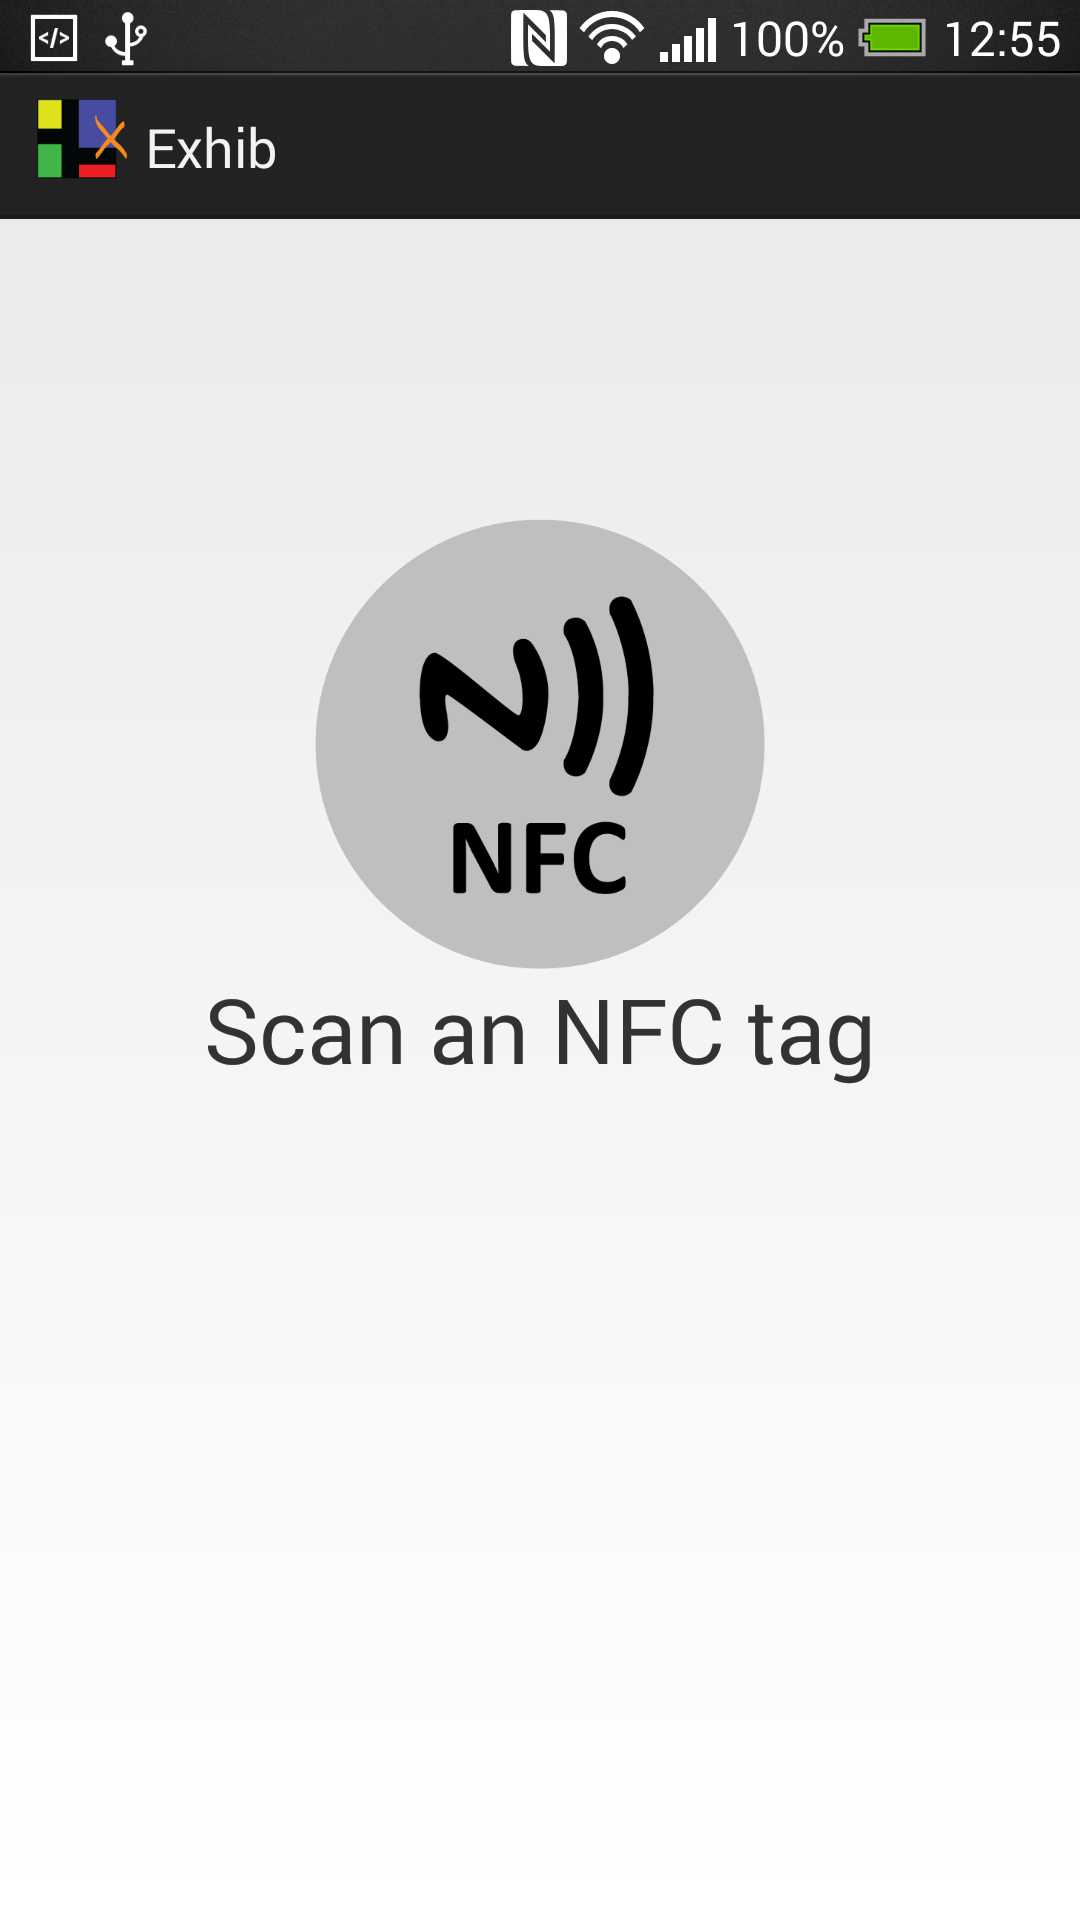
\includegraphics[width=0.7\columnwidth]{img/finaldesign/nfcscreen.png}
\caption{Start screen}
\label{fig:nfcscreen}
\end{minipage}
\hspace{0.5cm}
\begin{minipage}[b]{0.5\columnwidth}
\centering
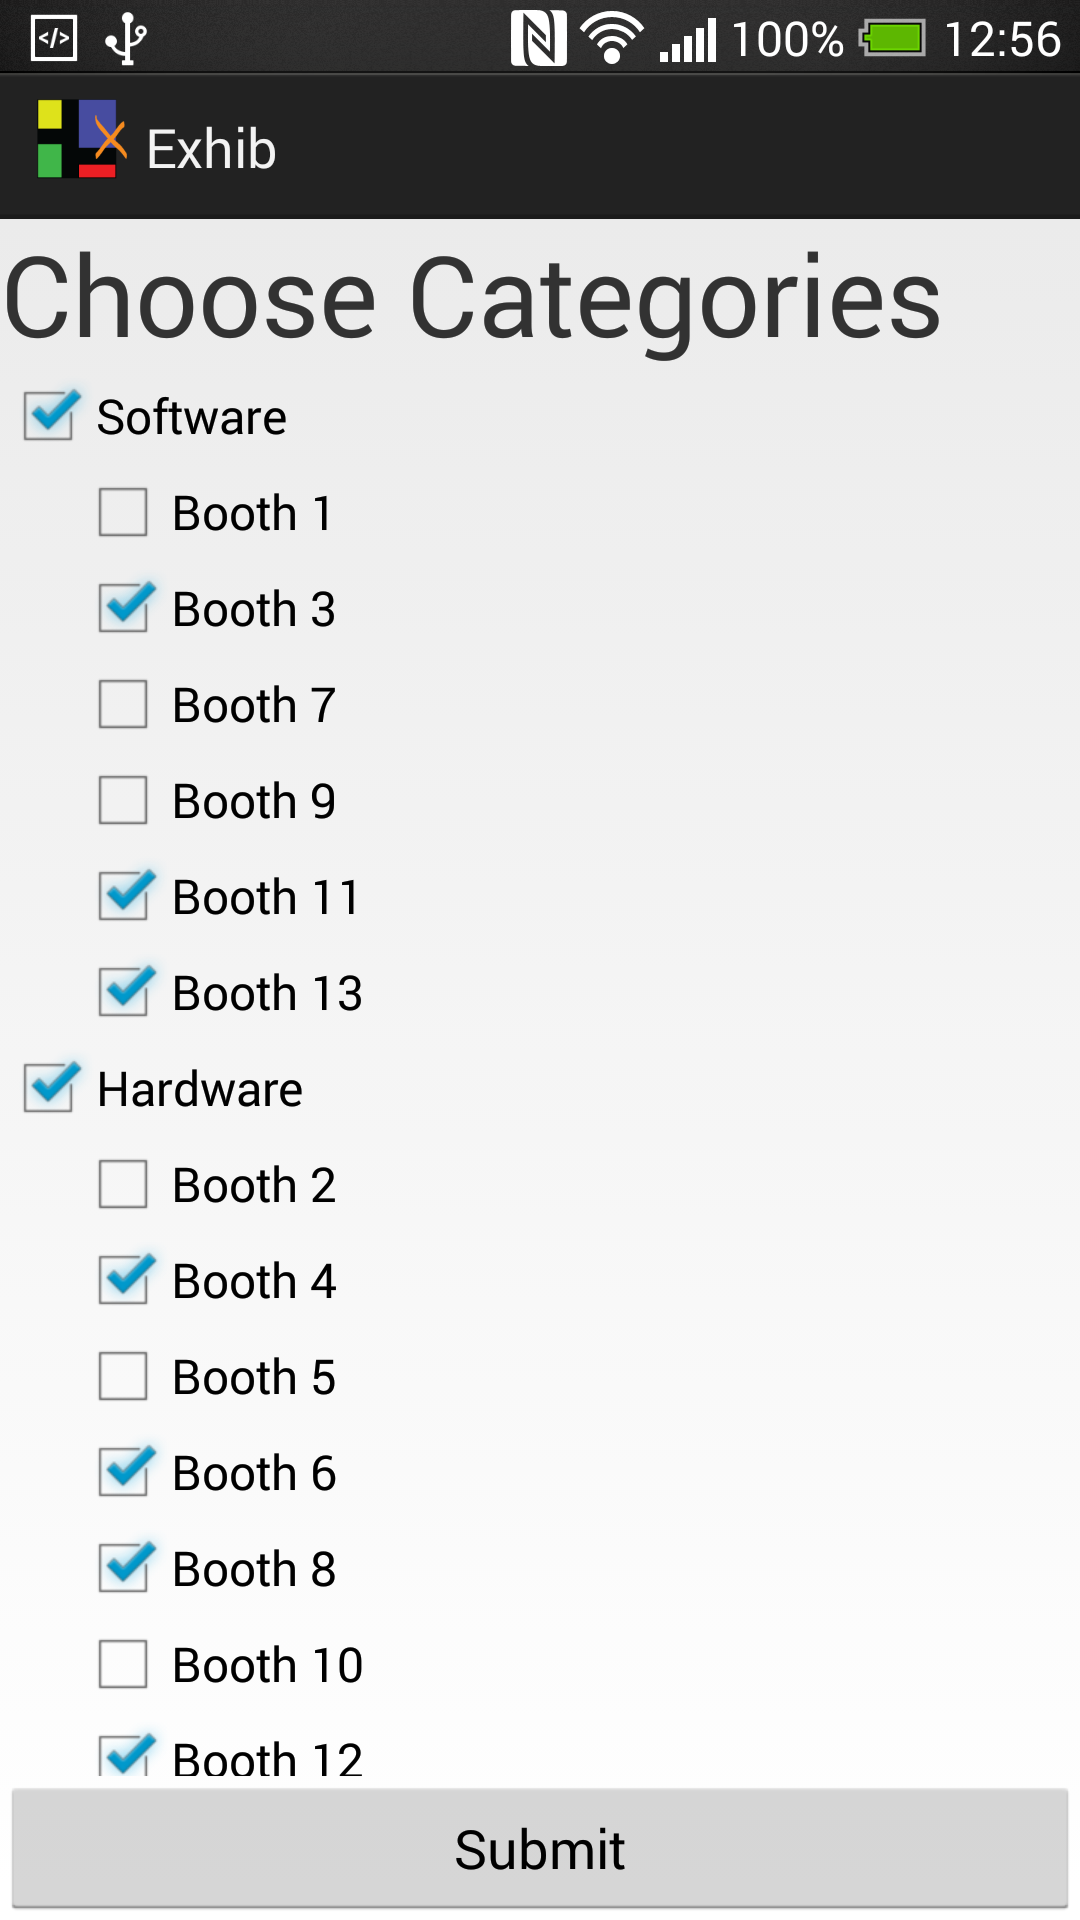
\includegraphics[width=0.7\columnwidth]{img/finaldesign/categories.png}
\caption{Categories}
\label{fig:categories1}
\end{minipage}
\end{figure}

When opening the application the first screen you encounter is one telling the user to scan an \ac{nfc} tag. The screen is shown on \autoref{fig:nfcscreen}. The windows differs from the prototype, as there is no menu in the bottom right to browse recent exhibitions. When the \ac{nfc} tag is scanned, you are signed up to that specific exhibition and a file with a pair of user ID and exhibition ID is saved on the phone, this will be explained in greater detail in the next section. A new screen appears asking the user to choose between different categories and booths, this is to identify the users interests which will be used later by the application. This is shown on \autoref{fig:categories1}. After the user has selected their categories, they press submit. 

\begin{figure}[H]
\begin{minipage}[b]{0.5\columnwidth}
\centering
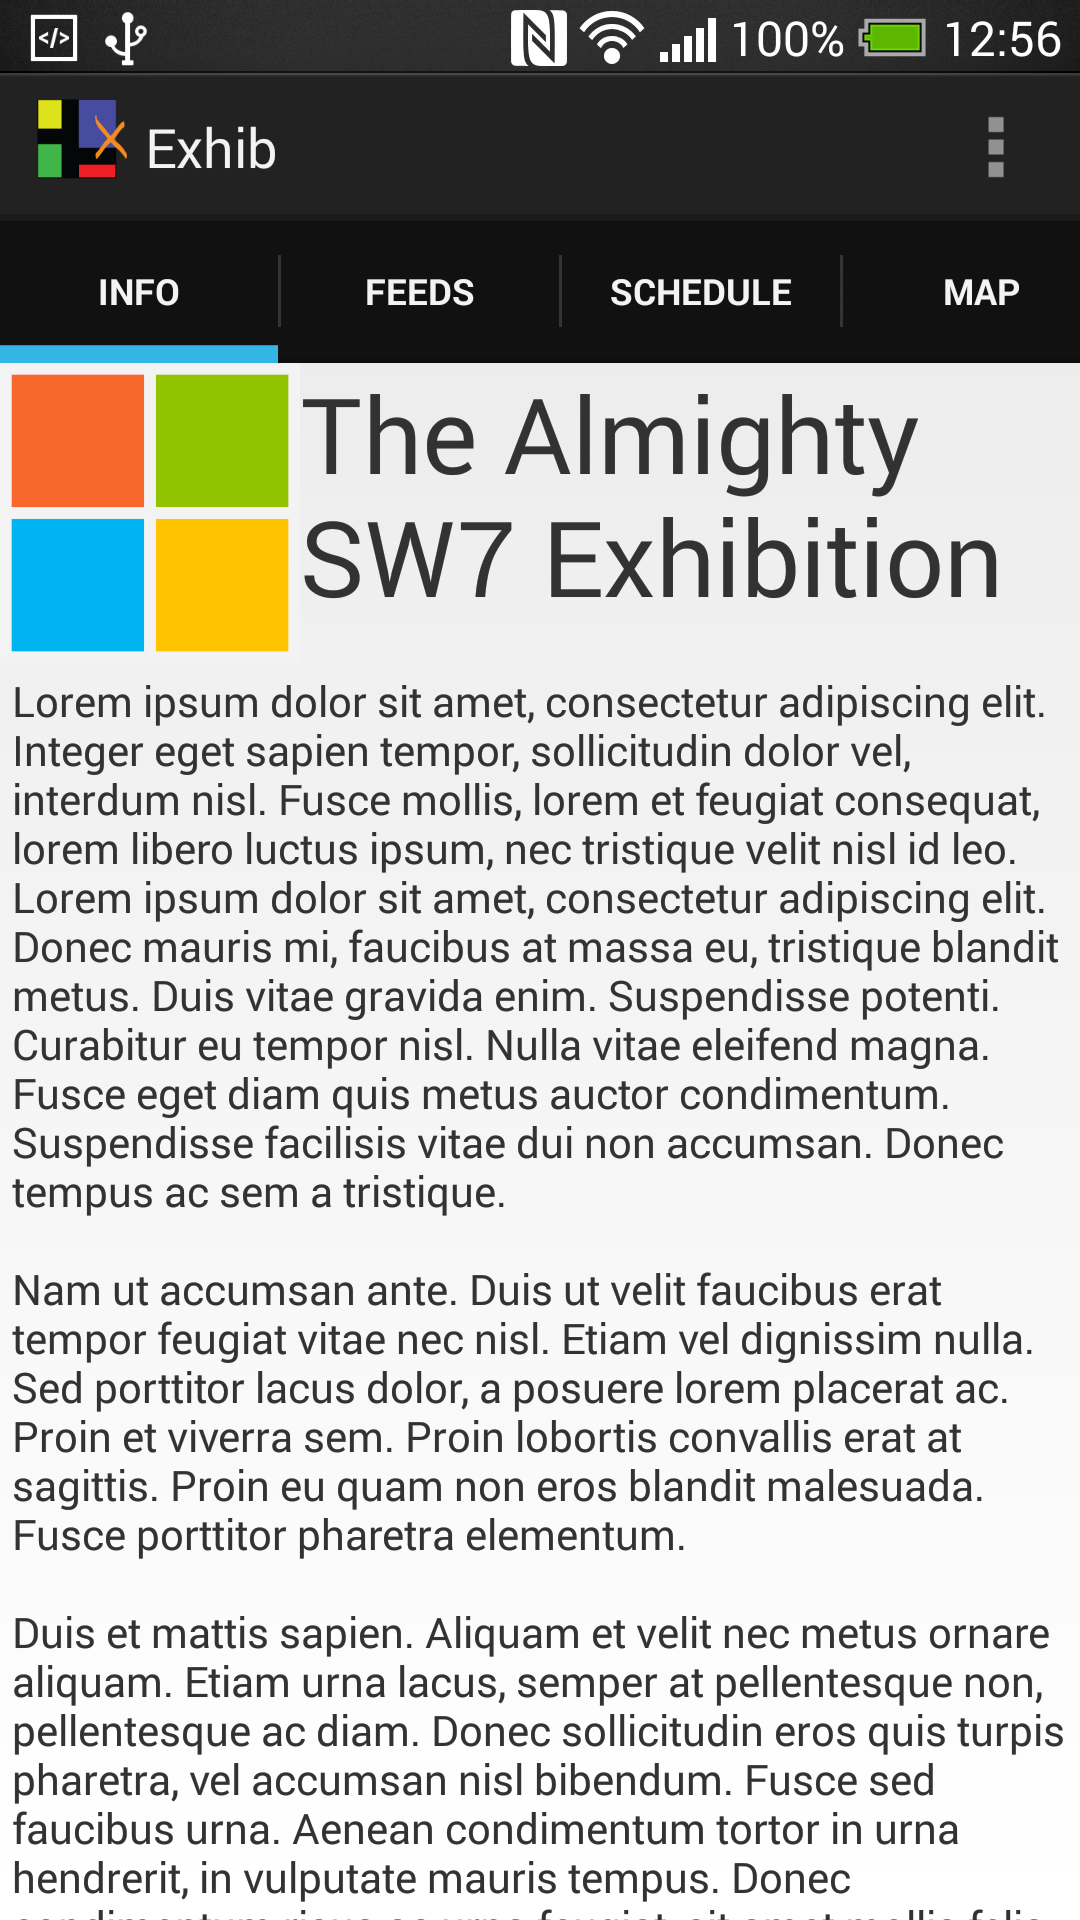
\includegraphics[width=0.7\columnwidth]{img/finaldesign/infoscreen.png}
\caption{Exhibition information}
\label{fig:infoscreen}
\end{minipage}
\hspace{0.5cm}
\begin{minipage}[b]{0.5\columnwidth}
\centering
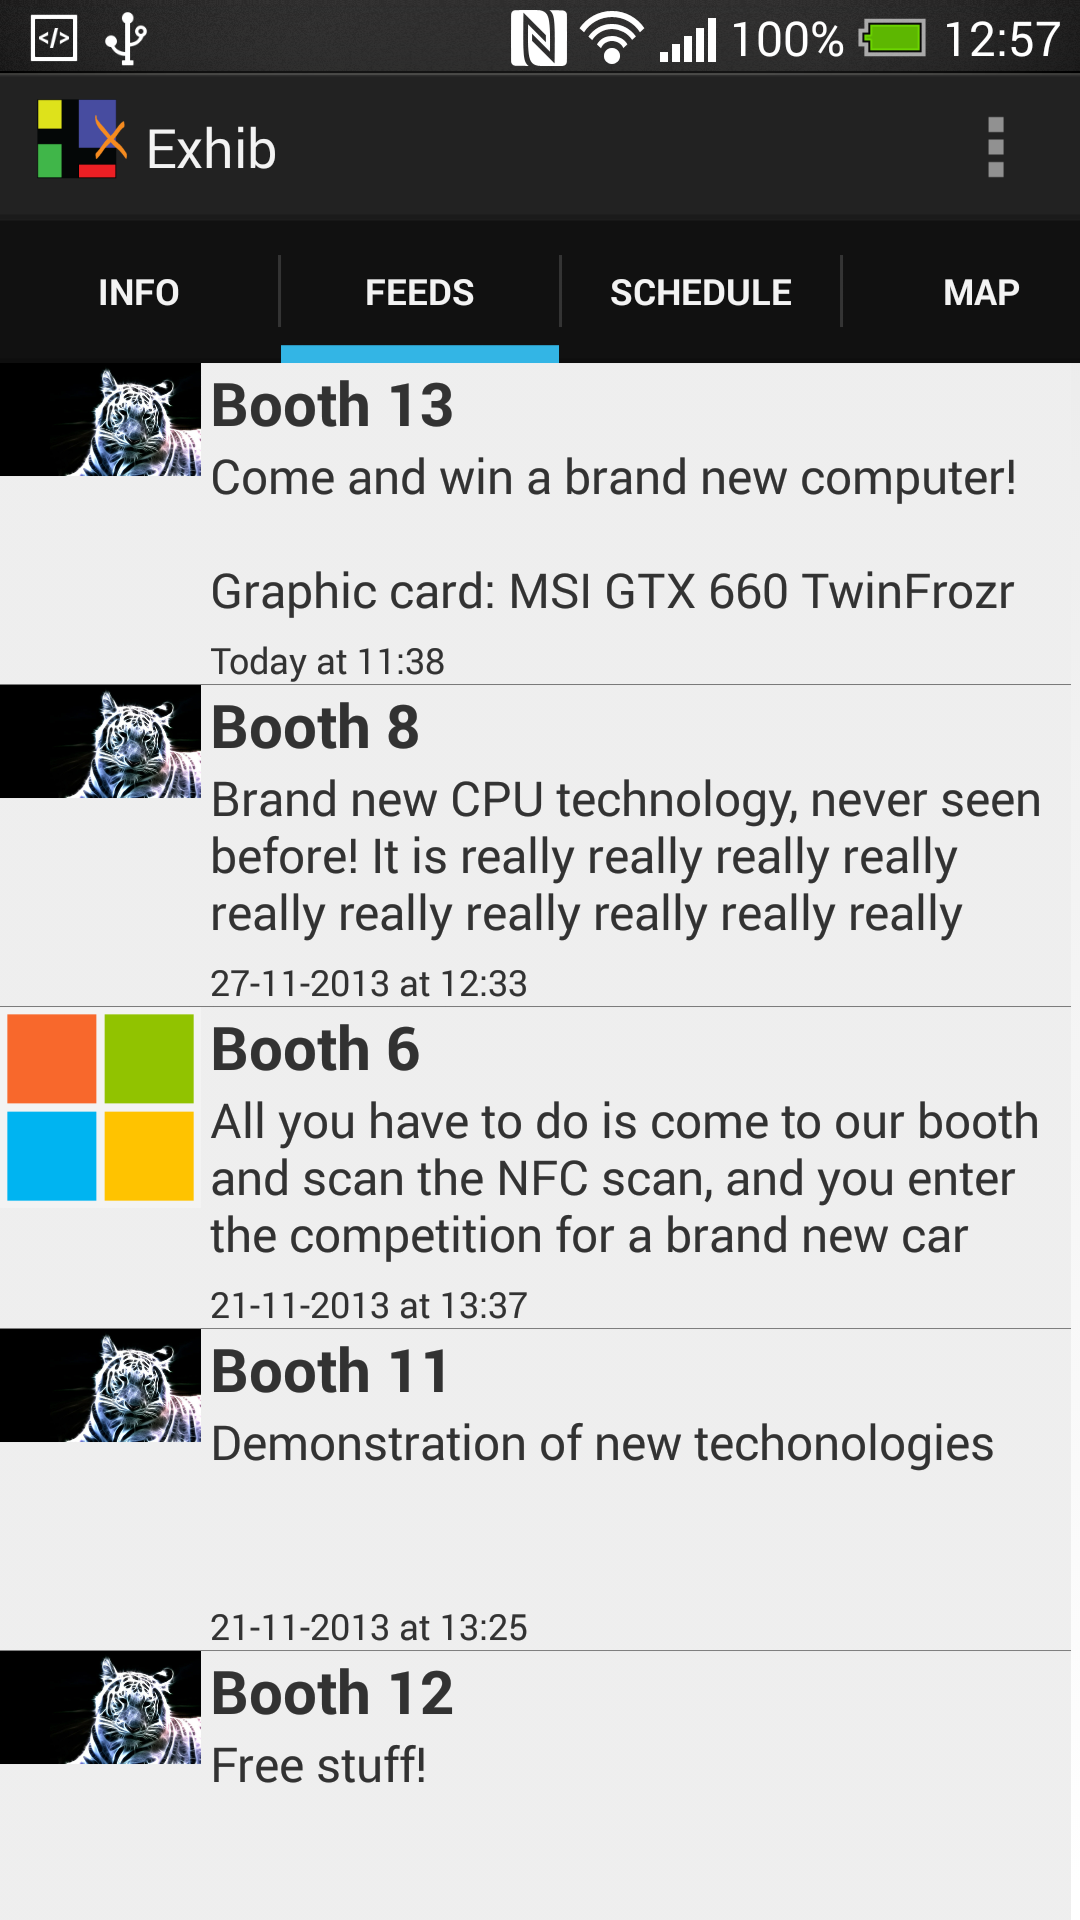
\includegraphics[width=0.7\columnwidth]{img/finaldesign/feedsscreen.png}
\caption{Feed list} 
\label{fig:feedsscreen}
\end{minipage}
\end{figure}

After having submitted the categories the user want to subscribe to, the user will be taken to an "Info" tab, this is a simple tab displaying information about exhibition the user are currently at, such as exhibition logo, name and a description of the exhibition. This can be seen on \autoref{fig:infoscreen}  at the top. Next to "Info" there are three other tabs: "Feeds", "Schedule", and "Floor Plan". These four tabs can be navigated to and from, from any of the other tabs either by swiping from side to side or by clicking on the tab itself at the top.

The tab "Feeds", as seen on \autoref{fig:feedsscreen}, shows a list feeds made by booths at the exhibition, note that the feeds do not have a header like shown on the prototypes. We decided against this because we felt it would take up too much space. The application uses the booths that the user subscribed to before, the user only receives feeds from the booths that they subscribed to after scanning the \ac{nfc} tag. Each feed has a timestamp telling the user when it was made.

It is also possible for the user to change the booths they have subscribed to, if they want to receive different feeds. This is done by pressing the three vertical dots in the top right corner, this takes they user to the categories screen again where they can choose new categories and booths. For some phones these dots will be located as a hardware button itself, and then the dots will not be in the application.

\begin{figure}[H]
\begin{minipage}[b]{0.5\columnwidth}
\centering
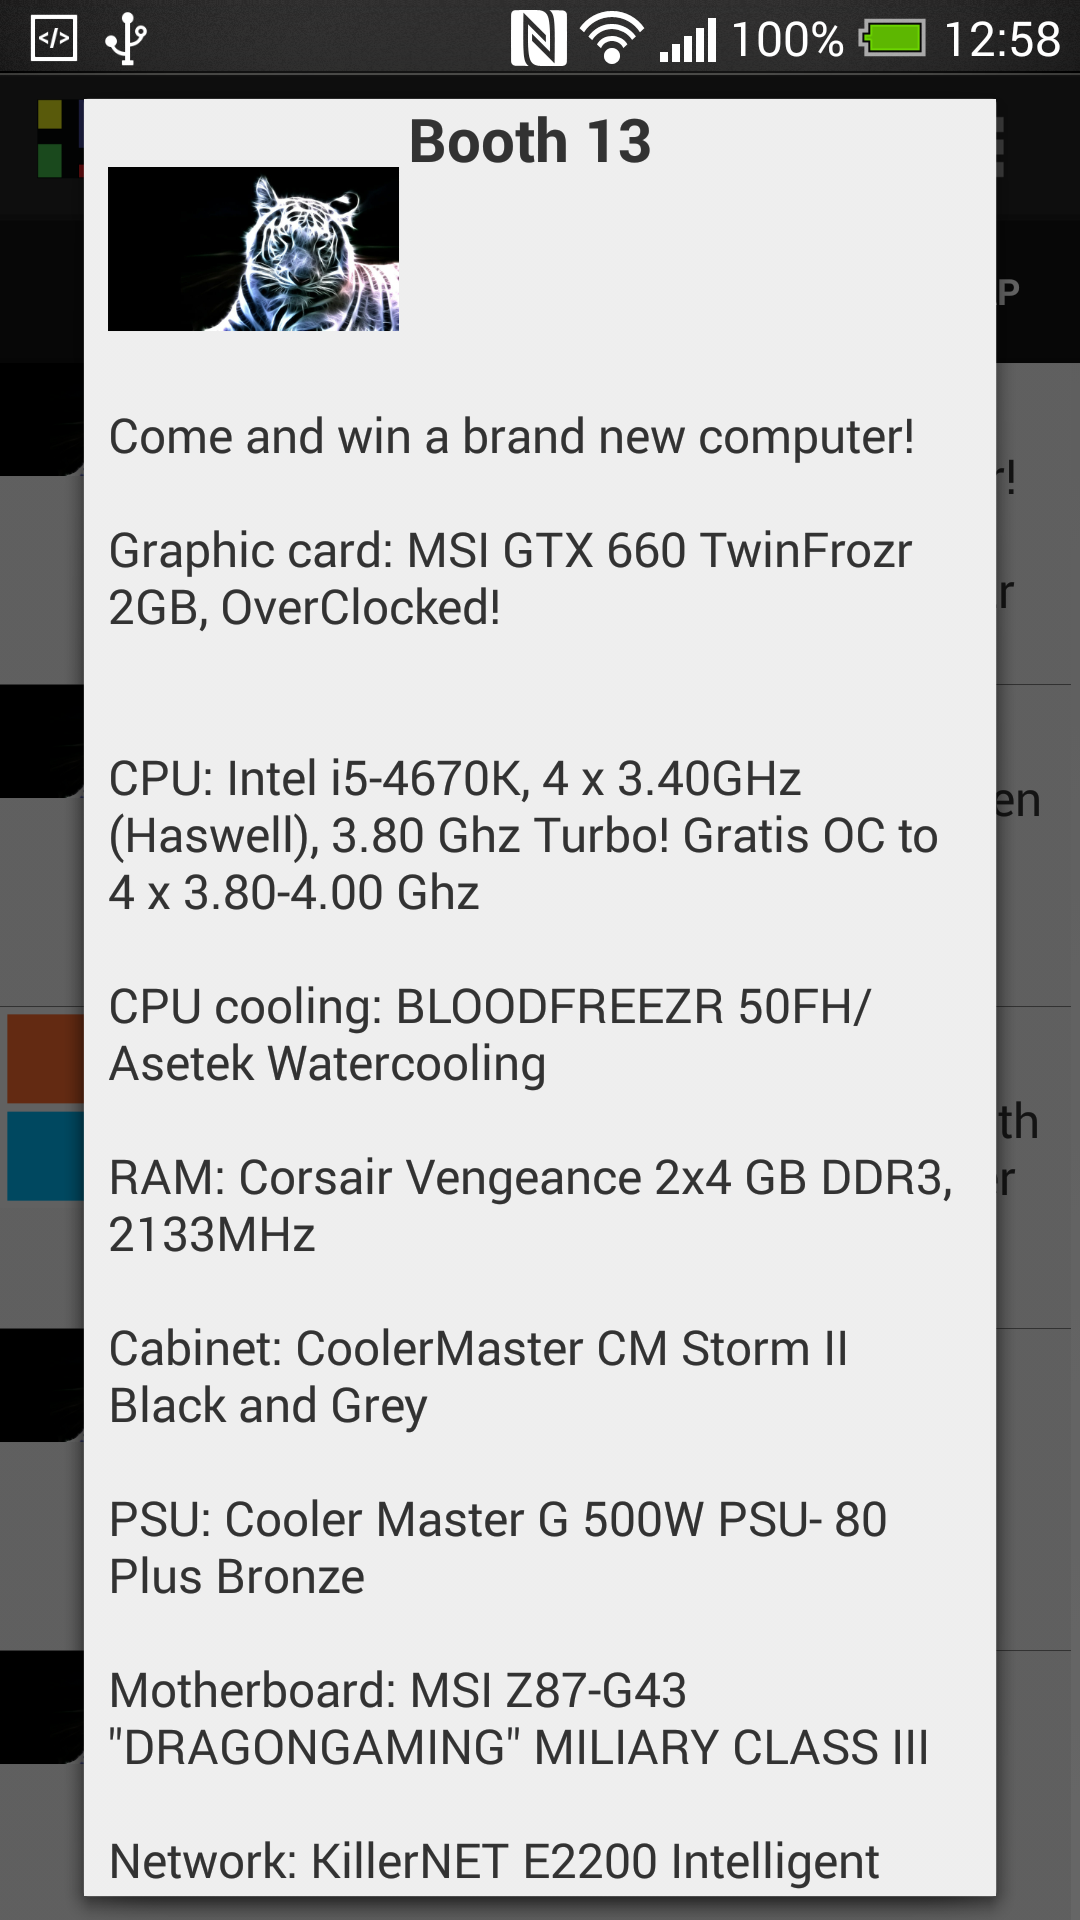
\includegraphics[width=0.7\columnwidth]{img/finaldesign/feedspopup.png}
\caption{Feed popup}
\label{fig:popupfeed}
\end{minipage}
\hspace{0.5cm}
\begin{minipage}[b]{0.5\columnwidth}
\centering
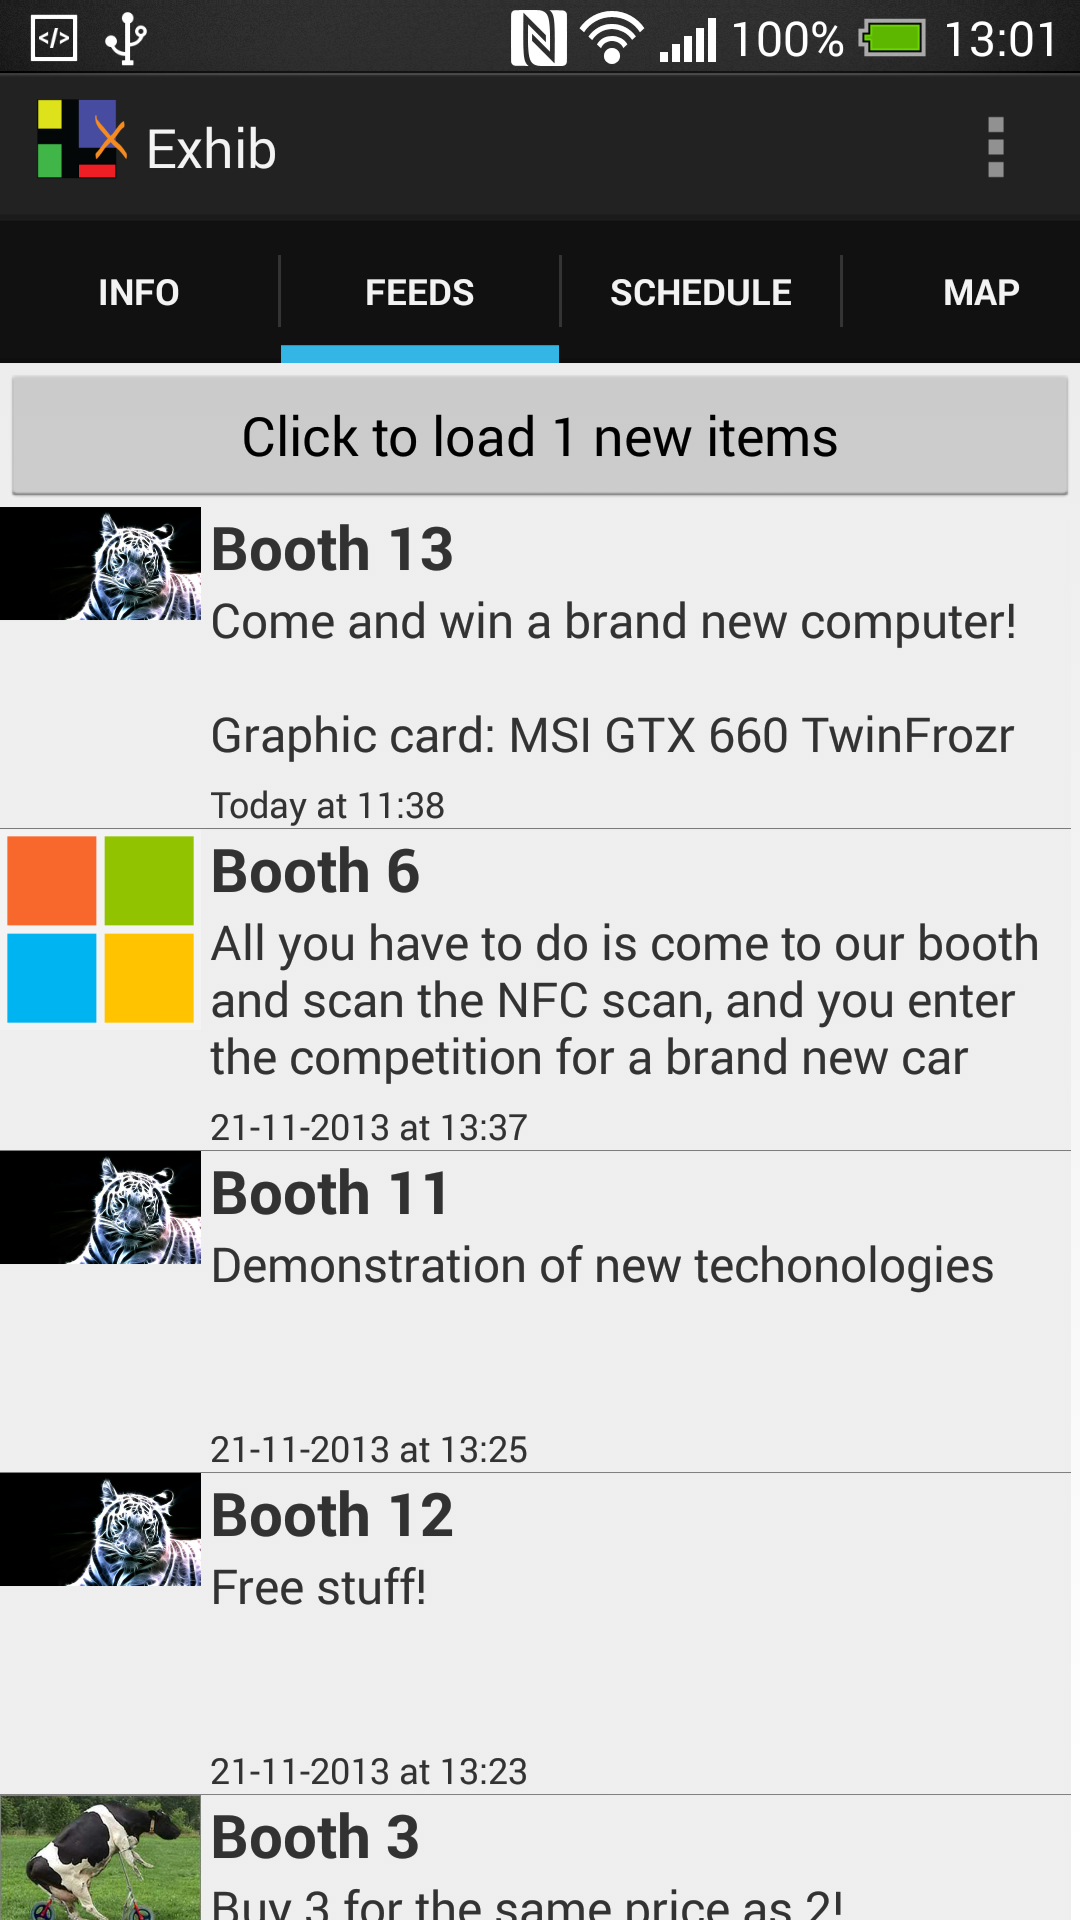
\includegraphics[width=0.7\columnwidth]{img/finaldesign/feedsnewitem.png}
\caption{New feed item}
\label{fig:feedsnewitem}
\end{minipage}
\end{figure}

Some of the feeds are too long to display all the text in the list of feeds, so in order to read the full feed you can press the feed and a pop-up will come up displaying the full feed, as shown on \autoref{fig:popupfeed}. This is different from the prototype, because we thought it would be more convenient for the user to have a pop-up. During the exhibition, the booths might send new feeds, when this happens a button will be displayed, telling the user that more feeds are available, allowing them to choose when they want to load the new feeds so they always can make sure they have read all feeds before loading new ones. This can be seen on \autoref{fig:feedsnewitem}. Note that this is only when the user has the feed list open, if they are on another tab or has the application closed, the new feeds will automatically be loaded.

\begin{figure}[H]
\begin{minipage}[b]{0.5\columnwidth}
\centering
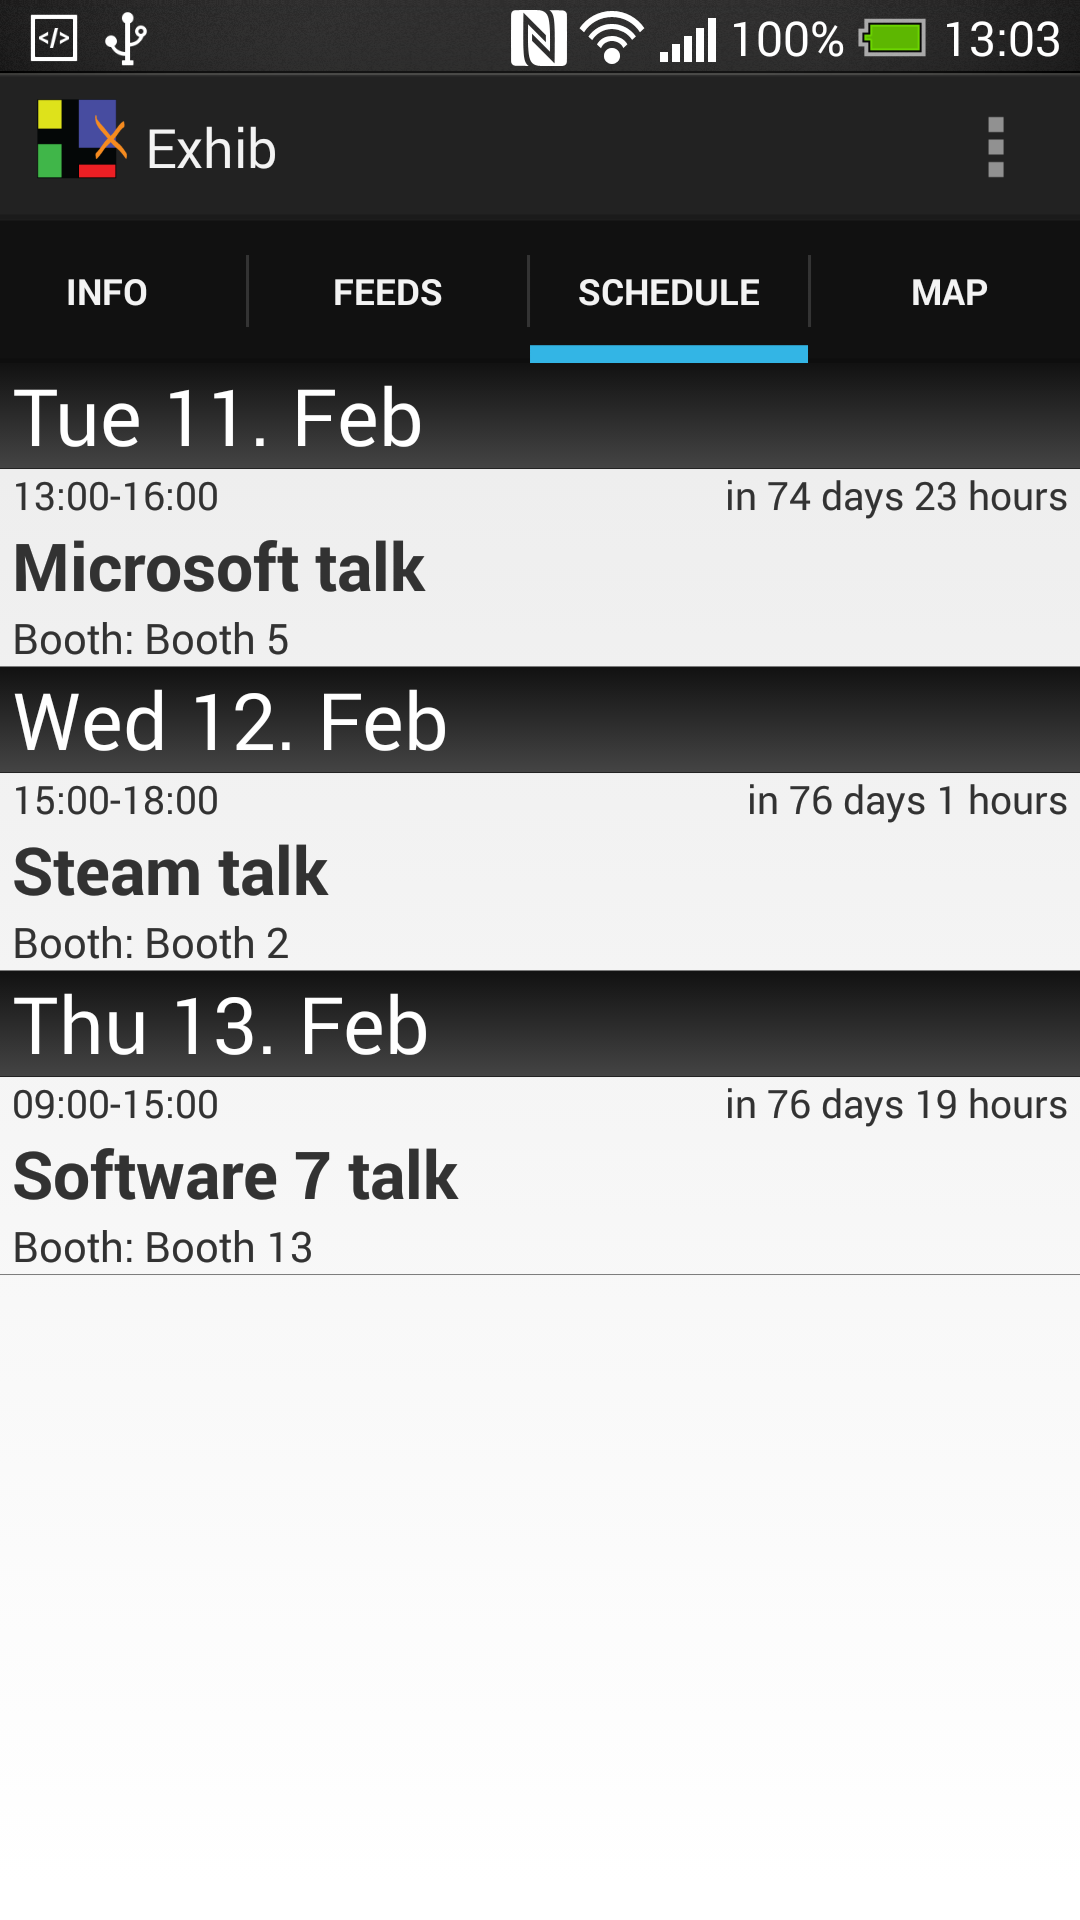
\includegraphics[width=0.7\columnwidth]{img/finaldesign/schedule.png}
\caption{Schedule}
\label{fig:schedule1}
\end{minipage}
\hspace{0.5cm}
\begin{minipage}[b]{0.5\columnwidth}
\centering
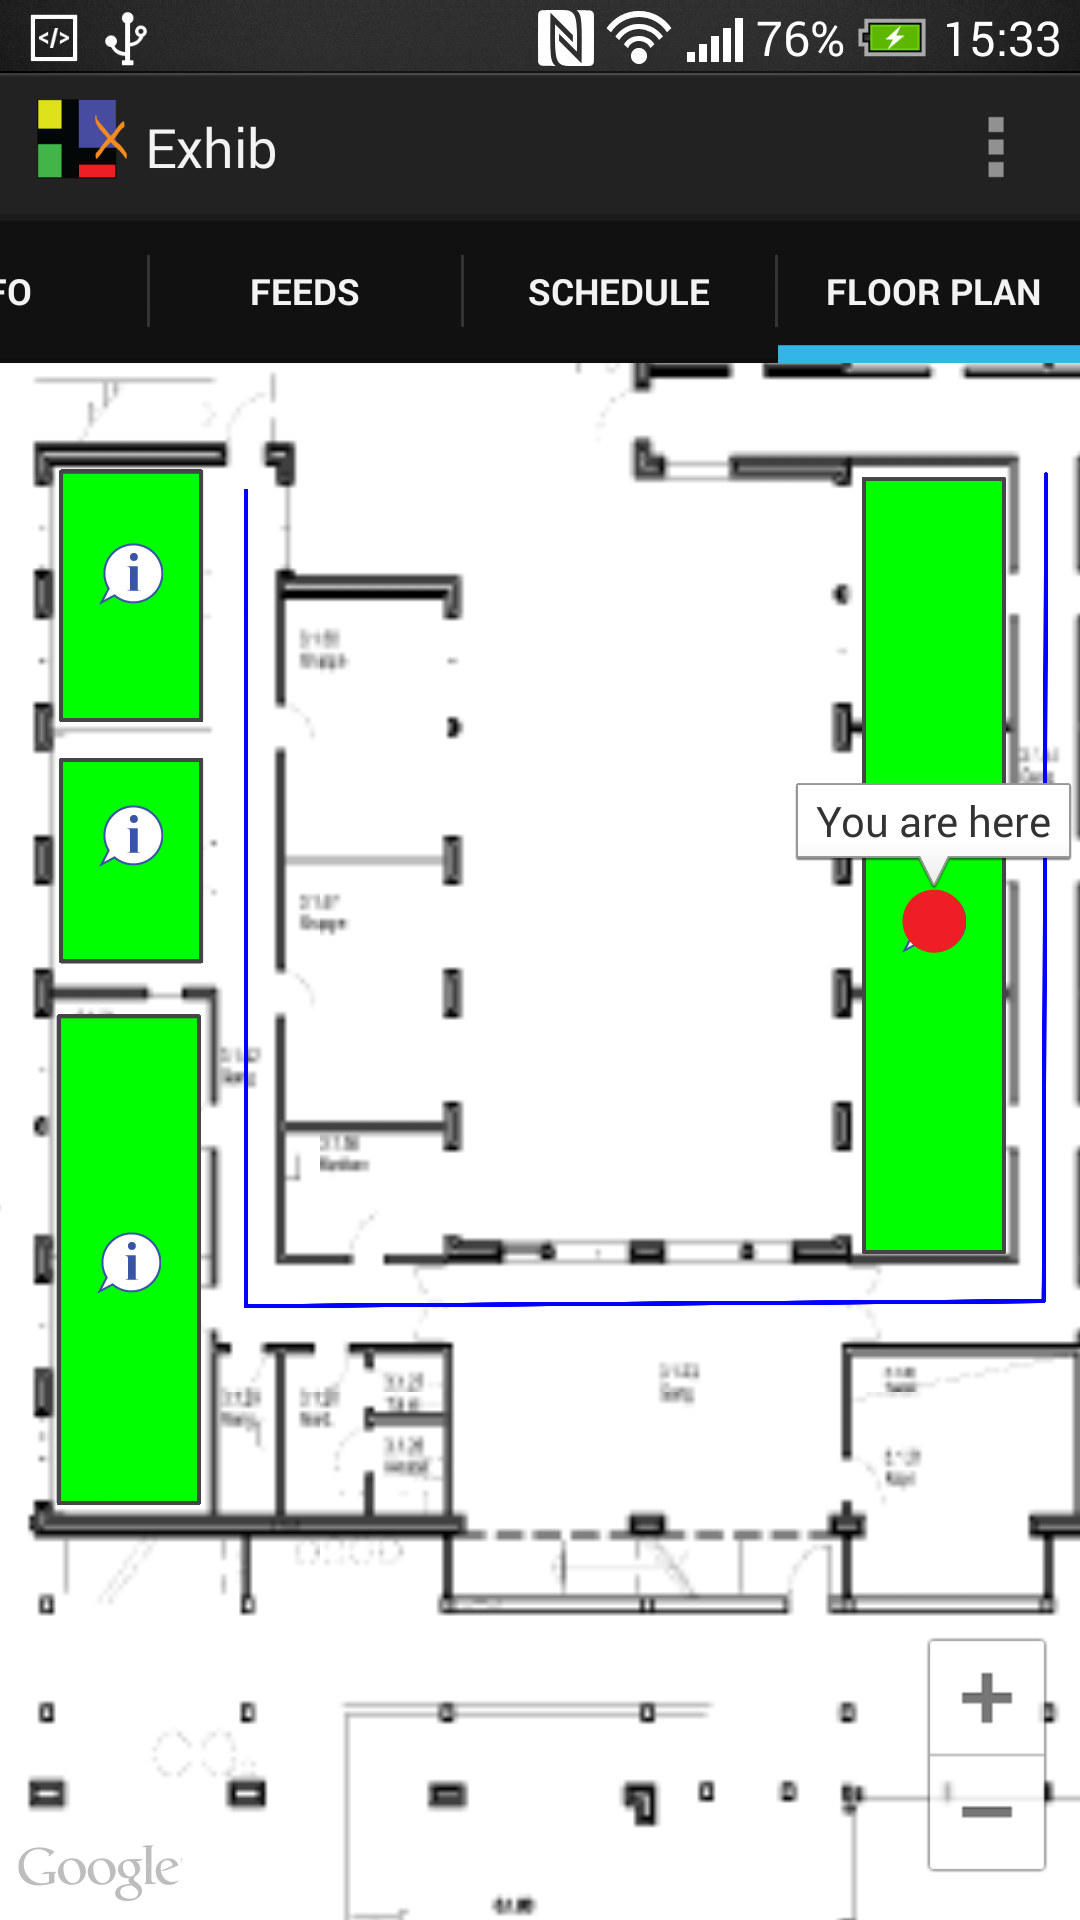
\includegraphics[width=0.7\columnwidth]{img/finaldesign/map1.png}
\caption{Floor plan}
\label{fig:map1}
\end{minipage}
\end{figure}

The "Schedule" tab shows the events that is going on at the exhibition itself, if the booths have a larger presentation they can add it to the schedule. This can be seen on \autoref{fig:schedule1}. Each event in the schedule has a countdown to when it will happen. 

The last tab is "Floor Plan", this is a map showing the exhibition with all its booths displayed. The blue line between the booths are the walk paths around the exhibition. If you scan an \ac{nfc} on one of the booths, the floor plan will snap to that booth on the floor plan and display a red circle to show where you are. It also snaps to this booth. This is seen on \autoref{fig:map1}. 

\begin{figure}[H]
\centering
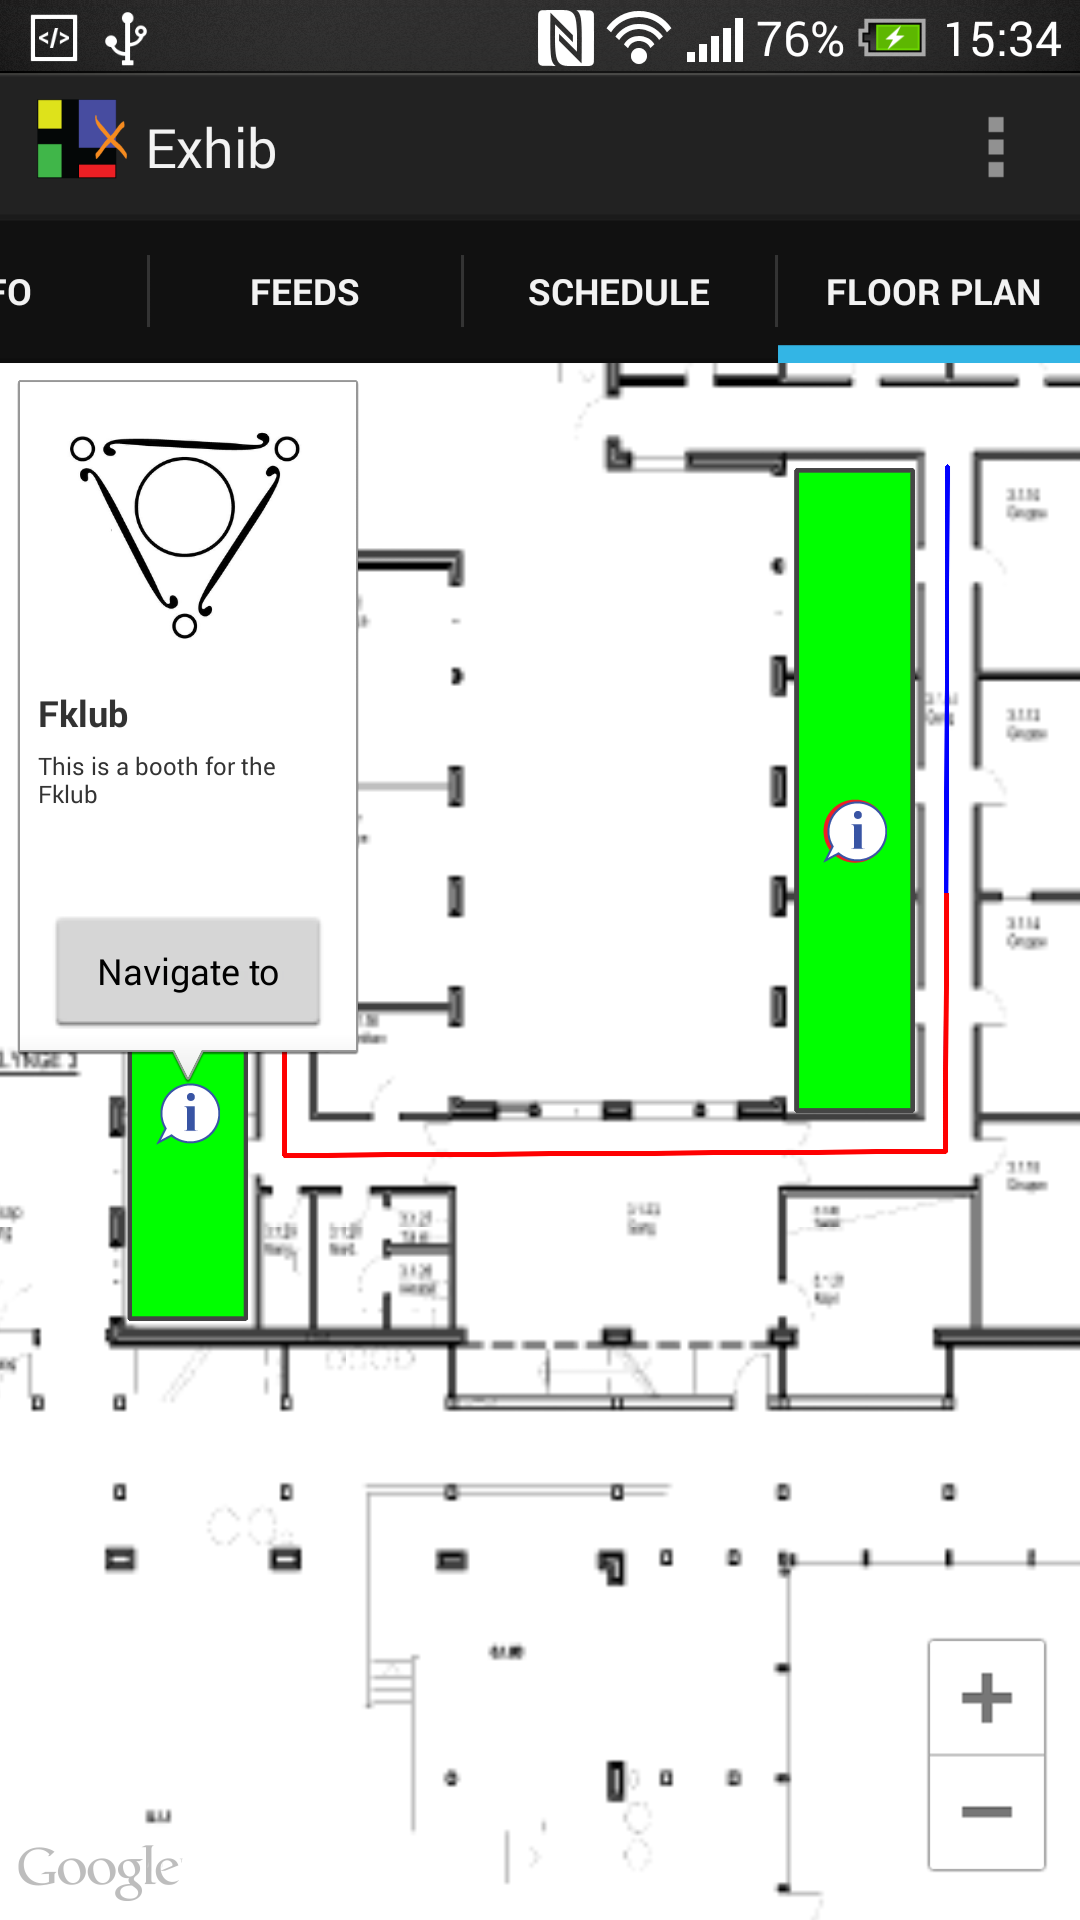
\includegraphics[width=0.35\columnwidth]{img/finaldesign/map2.png}
\caption{Floor plan with booth}
\label{fig:map2}
\end{figure}

You can also press the info icon on each booth, to receive information about this booth, this is seen on \autoref{fig:map2}. Note the "Navigate to" button, this allows the user to get a route from their last scanned booth and to the booth of their choice. If the user chooses to navigate to a specific booth, the walk path from their current position and to the booth will be highlighted with red instead of blue. This can also be seen on \autoref{fig:map2}. Note that unlike the prototype, the "Floor Plan" tab does not have a "lock" button, instead the whole tabs locks automatically when swiped to and the user has to press one of the other tabs in order to change tabs.

\autoref{fig:flowchart} shows the application flow between these different activities. Note that the \textit{TabActivity} consists only of tabs, each tab is defined in a fragment.

\begin{figure}[H]
\centering
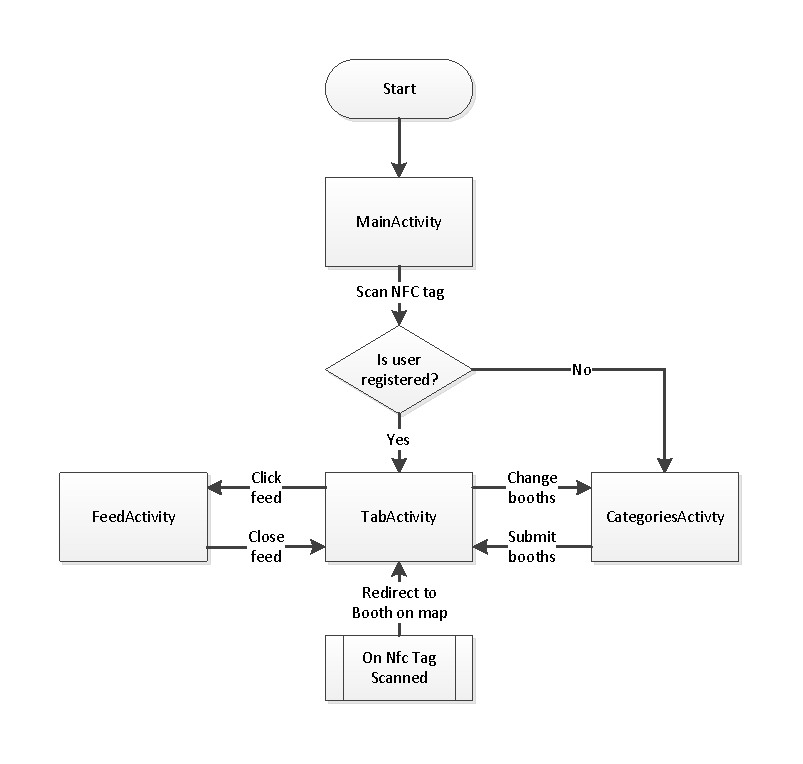
\includegraphics[width=\columnwidth]{img/appFlowchart.pdf}
\caption{Application actvity flow\label{fig:flowchart}}
\end{figure}
\todo{Pictures and description of the finished application}

\section{User ID}
As mentioned in the previous section, when scanning an \ac{nfc} tag for the first time the user has to choose booth subscriptions. After having chosen these subscriptions, the user ID, the exhibition ID and the IDs of the subscribed booths are saved to the database. A user for this exhibition is now created. If scanning another tag, two different scenarios can occur;
\begin{description}
\item[Same ID] Scanning a tag with the same exhibition ID as the first one you scanned, the application will search the file for the matching pair of user ID and exhibition ID and request the IDs of the booths that the user has subscribed to from the database, this means that the user will not have to choose subscriptions again and is taken directly to the tab activity of the recently scanned exhibition. 
\item[Different ID] If the exhibition ID does not match the one in the file, then a new user ID and exhibition ID is saved to the file and you are asked to subscribe to booths at the new exhibition. 
\end{description}
If the user opens up the application without scanning a tag then they are taken to the tab activity of the most recent exhibition. 

If a user deletes the application, the file is deleted as well which means the user loses their user ID. Due to our application not having any login system requiring username and password, the only data that is lost is their booth subscriptions. Next time they install the application and scan a tag they will be assigned a new user ID and have to choose booth subscriptions again.

\section{System Architecture}

\begin{figure}[H]
\centering
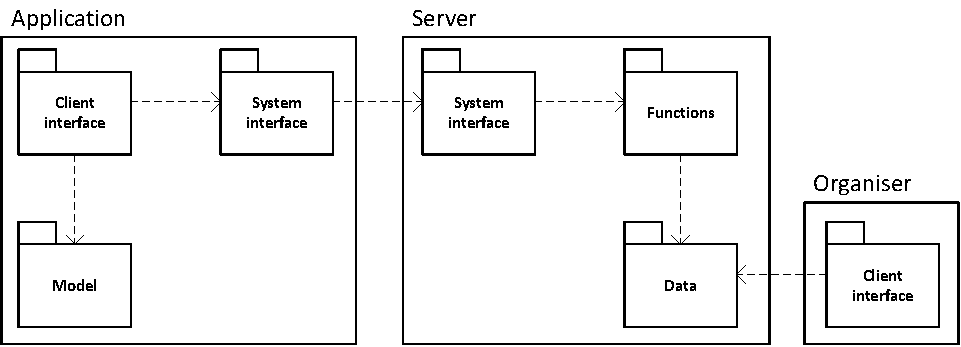
\includegraphics[width=\linewidth]{img/components.pdf}
\caption{System architecture\label{fig:architecture}}
\end{figure}

\autoref{fig:architecture} shows the architecture of the entire system. The application only has a \textit{Model} component which contains simple classes for feeds, schedule items, etc. The application does not have a \textit{Functions} component because most of the functionalities are provided by the server's functions. The organiser i.e. the website, currently alters the data component directly. A better solution would be to only let the server \textit{Functions} alter the data in order to encapsulate the it.
